% !TeX root = ../main.tex
% Add the above to each chapter to make compiling the PDF easier in some editors.

\makeatletter
\renewcommand{\maketitlepage}{%
    \cleardoublepage{%
        \begin{fullwidth}%
        \fontsize{12}{12}\selectfont\par\noindent{\@author \\ \noindent \small{based on a lecture of Frank Himstedt}}%
        \vfill
        \begin{figure}
            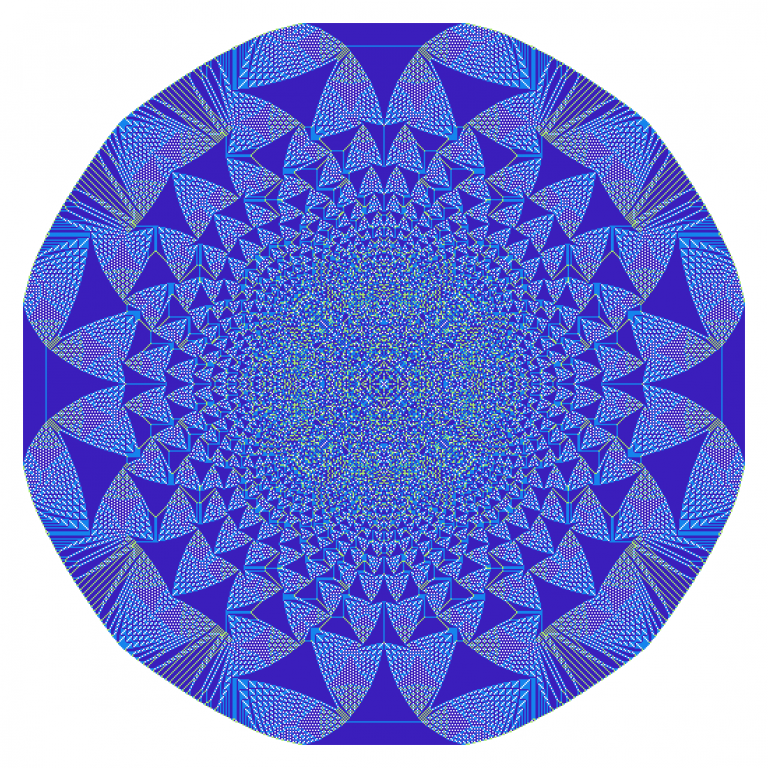
\includegraphics[width=10cm]{figures/cover.png}
            % \caption{Caption}
        \end{figure}
        \fontsize{40}{46}\selectfont\par\noindent{Abstract Algebra}%
        % \fontsize{14}{16}\selectfont\par\noindent\@date
        % \vspace{5.5pc}%
        \vfill
        % \fontsize{14}{16}\selectfont\par\noindent\thanklesspublisher%
        \fontsize{10}{12}\selectfont\par\noindent{\textbf{Contents.} Groups, homomorphisms, cyclic groups, Sylow theorems, and solvable groups. Rings, ideals, polynomial rings, irreducibility of polynomials. Fields, field extensions, Galois theory, solvable polynomials.} \\[5pt]
        \fontsize{10}{12}\selectfont\par\noindent{Illustration is due to Katherine E. Stange.}\par\noindent{Contributions are welcome at \url{https://github.com/jonhue/algebra}.}
        \end{fullwidth}%
    }%
    \thispagestyle{empty}%
    \clearpage
}
\makeatother
